\subsection{Mobility detection}
\label{subsec:reverse-tt}

Mobility detection is a key issue to handle mobile nodes on $\mu$Matrix. If nodes by itself inform its motion (e.g. by using accelerometer or GPS) to the protocol, then we refer to as active motion, otherwise if the protocol infer the node movement, we refer to passive motion.

Trickle~\cite{Levis:2004} algorithm passively detects topology changes. However, Trickle lacks in agility to detect changes in dynamic network and mobile nodes. We propose Reverse Trickle timer that operates similarly to the standard algorithm, but in reverse order. 

\begin{figure}[t!]
\centering
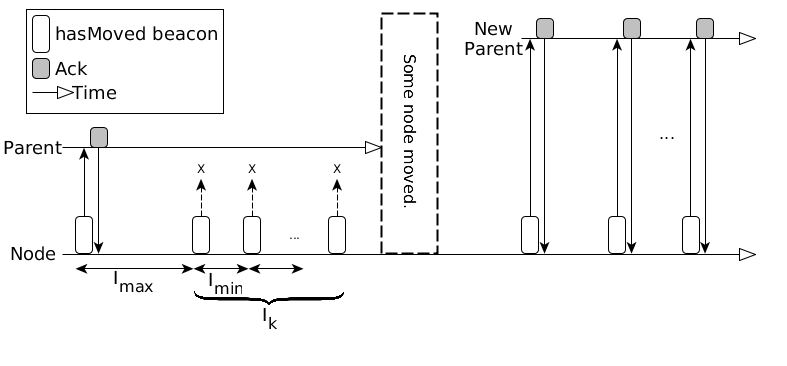
\includegraphics[width=1\linewidth]{img/reverse-tt}
\caption{Reserve Trickle timer operation.}
\label{fig:reverse-TT}
\end{figure}

Reverse Trickle introduce a control message and three parameters: 
\begin{inparaenum}[i)]
    \item \texttt{hasMoved} beacon;
    \item $I_{max}$ and $I_{min}$ the maximum and minimum time interval to send a \texttt{hasMoved} beacon;
    \item $I_k$ the number of attempts to query a node before declaring a inconsistency.
\end{inparaenum}
These parameters must defined by the network operator before.

Figure~\ref{fig:reverse-TT} shows the Reverse Trickle procedure. First, a node starts sending unicast \texttt{hasMoved} beacons to its parent. $I_{max}$ is the interval between two consecutive \texttt{hasMoved}. If the node did not receive an ack for a \texttt{hasMoved} beacon, then it sets the interval to $I_{min}$. After $I_k$ unsuccessful attempts, the node knows that someone moved. Thus, the node can take actions, for example, properly perform a handover to another parent and then the procedure restarts. Note that by setting the Reverse Trickle parameters, the network operator should consider the trade-off between delay to detect mobility and number of beacons. For a smaller delay to mobility detection, $I_{max}$ must be tuned to small values at cost of more \texttt{hasMoved} beacons. In our experiments (Section~\ref{sec:evaluation}) reverse trickle parameters were set according to application data rate (Table~\ref{tab:sim-params}). 

In \cite{oliveira2016low}, the authors argue that a common modification to support mobility is change the control message periodicity. The typical approach uses a simple periodic timer or the standardized Trickle timer. While reverse trickle waits for $I_{max} + T_k \times I_{min}$ to detect a topology change, where $I_{min} \ll I_{max}$, the periodic and standardized Trickle approaches wait for at least $2\times I_{max}$.  